% This is the template Jun uses for project seeds
% jun.allard@uci.edu allardlab.com
\documentclass[onecolumn,11pt]{article}

% --------- required packages ---------
\usepackage{enumerate}
\usepackage{enumitem}
\usepackage{graphicx}
\usepackage[colorlinks,allcolors=black]{hyperref}
\usepackage[font=small]{caption}
\usepackage{siunitx}
\usepackage{times}
\usepackage{titlesec}

\usepackage{titling}
\usepackage{authblk} % must come after titling package loading

% --------- standard packages ---------
%\usepackage{amsfonts}
\usepackage{amsmath}
\usepackage{amssymb}
%\usepackage{array}
%\usepackage{bm}
%\usepackage{color}
%\usepackage{chemarr}
%\usepackage{float}
\usepackage[utf8]{inputenc}
\usepackage{lipsum}
%\usepackage{mathtools}
%\usepackage{multicol}
%\usepackage{multirow}
%\usepackage{pdfsync}
%\usepackage{tocloft}
%\usepackage{verbatim}
%\usepackage{wrapfig}


% --------- packages, less often used ---------
%\usepackage[export]{adjustbox}
%\usepackage{amsopn}
%\usepackage{cancel} % adds strikethrough
%\usepackage{CJK} % Chinese Japanese Korean
%\usepackage{dcolumn} % align columns in a table
%\usepackage{dsfont}
%\usepackage{epsfig}
%\usepackage{epstopdf}
%\usepackage{esint} % integrals
%\usepackage{framed}
%\usepackage{physics} %for \vqty, \dd, \dv
%\usepackage{rotating}
%\usepackage{setspace} % set space between lines
%\usepackage{subcaption}
%\usepackage{tcolorbox}
%\usepackage[normalem]{ulem} % for underlining
% --------- for typesetting code blocks --------
%\usepackage{algorithmic} % for code including Matlab
%\usepackage{listings} % for code including Matlab
%\usepackage[numbered,framed,basicstyle]{matlab-prettifier}

%%%%%%%%%%%%%%%%%%%%%%%%%%%%%%%%%%%%%%%%%%%%%%%%%%%%%%%%%%%%
% page layout
\usepackage[margin=1in]{geometry}

% paragraph layout
\setlength{\parindent}{0pt} % paragraph indent - looks best zero
\setlength{\parskip}{0.8em plus 0.1em minus 0.1em} % paragraph spacing
\setlist[itemize]{itemsep=0.0em,topsep=0em}
\setlist[enumerate]{itemsep=0.0em,topsep=0em}
\titlespacing{\paragraph}{0em}{-0.8em}{1em} % for the /paragraph command

% Bibliography setup
\usepackage[numbers,square,sort&compress]{natbib}
\bibliographystyle{unsrtnat}
%\bibliographystyle{biophysj}

\title{Project JeanJacket}
\author[a]{Jun}
\affil[a]{University of California Irvine}


%%%%%%%%%%%%%%%%%%%%%%%%%%%%%%%%%%%%%%%%%%%%%%%%%%%%%%%
\date{} % leave blank for no date
\begin{document}

\maketitle
%%%%%%%%%%%%%%%%%%%%%%%%%%%%%%%%%%%%%%%%%%%%%%%%%%%%%%%

%\begin{abstract}
%Nothing here yet
%\end{abstract}


\section{Project seed}

\subsection*{Summary}
\paragraph{Background/major question} \lipsum[2]
\paragraph{Specific question, puzzle or hypothesis}\lipsum[2]
\paragraph{Here we}\lipsum[2]
\paragraph{Methods, tools, expertise, skills}\lipsum[2]
\paragraph{Expected results}\lipsum[2]
\paragraph{Outcomes and implications}\lipsum[2]


%%%%%%%%%%%%%%%%%%%%%%%%%%%%%%%%
\begin{figure}[h!]
\centering
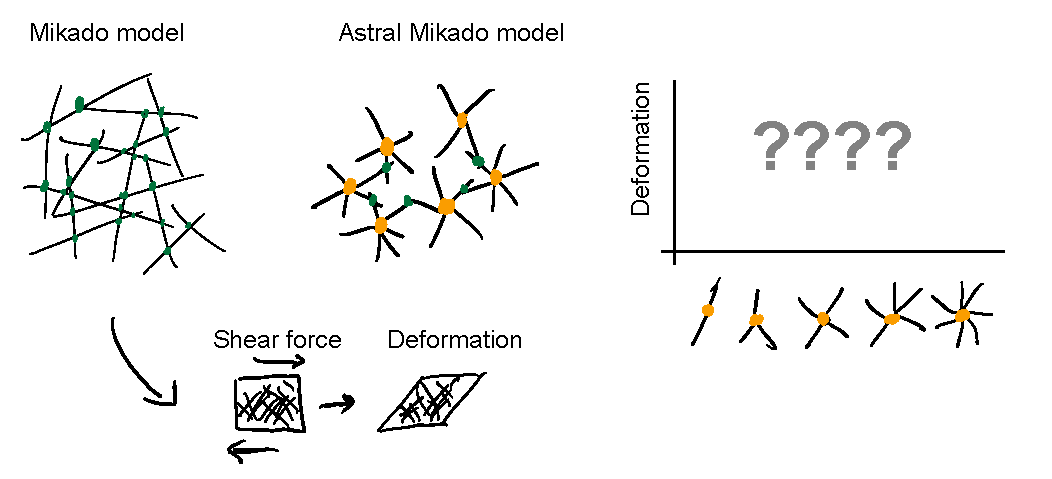
\includegraphics[width=4.5in]{figJeanJacket.pdf}
\caption{An awesome model of a puzzling phenomenon}
\label{fig:JeanJacketSchematic}
\end{figure}
%%%%%%%%%%%%%%%%%%%%%%%%%%%%%%%%

\subsection{Candidate titles}

\begin{itemize}
\item Predictive dynamic modeling connects timescales of day-to-day gene expression and decade-scale disease progression of Alzheimer's Disease using $\mathbb{C}^\star$ algebras
\item Ito lemma and Boltzmann statistics provide a cost-effective treatment for cardiovascular disease
\item Hybrid Metropolis-Gillespie algorithm reveals a novel design for enhanced CAR-T therapy by dynamnic recruitment of non-effector molecular crowders to the T cell membranes
\item Comparative study of noncanonical protrusions and what they optimize
\item Accelerated tendon healing by morphological alterations to tenocyte projections
\end{itemize}

\subsection*{Basic model}

\lipsum[2-5]

\subsection*{Reading}
Papers marked with $^{\bullet}$ are of notable interest.
\begin{itemize}
\item Primarily modeling: \citet{Slaughter.2013}, \citet{Zhang.2019}
\item Review articles on the system
\item Primarily experimental
\end{itemize}


\subsection*{First steps}

Dimensional analysis. Pull the other cell with \SI{10}{\pico\newton \per \second}. Deviatoric stress \SI{7e3}{\pascal}. Inside a math environment $R=\SI{120}{\micro\meter}$.


% Bibliography
\bibliography{jeanjacket}

%%%%%%%%%%%%%%%%%%%%%%%%%%%%%%%%%%%%%%%%%%%%%%%%%%%%%%%%%%%%%%%%%%%%%%%%%%%%%

% Supplemental
\clearpage
\setcounter{table}{0}
        \renewcommand{\thetable}{S\arabic{table}}%
\setcounter{figure}{0}
        \renewcommand{\thefigure}{S\arabic{figure}}%
\renewcommand{\listfigurename}{List of Supporting Figures}
\renewcommand{\contentsname}{List of Supporting Text}

%\section{Supplemental material}

%%%%%%%%%%%%%%%%%%%%%%%%%%%%%%%%
%\begin{figure}[h!t]
%\centering
%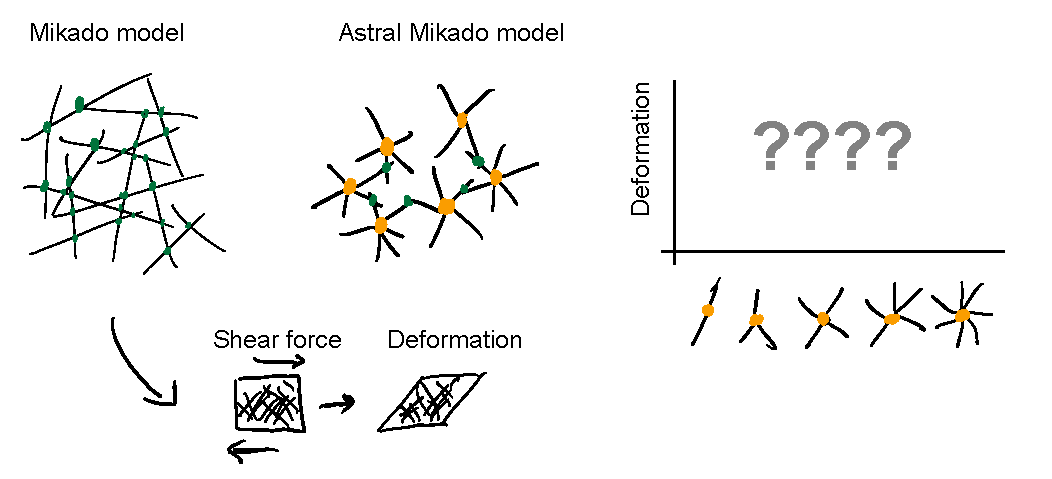
\includegraphics[width=4.5in]{figJeanJacket.pdf}
%\caption{This is a supplemental figure}
%\label{fig:DetailedJeanJacketSchematic}
%\end{figure}
%%%%%%%%%%%%%%%%%%%%%%%%%%%%%%%%

\end{document}
